\section{问题分析与总体思路}

\subsection{问题之间的逻辑关系}

第一问包含预测与识别两个不同任务。油价预测检验模型能否利用截止日前信息降低样本外
误差；事件研究检验冲突发生后是否出现相对历史规律异常的收益与波动。预测残差本身不能
被解释为战争的净因果贡献。进一步地，同样的油价上涨可能源于供给收缩、全球需求扩张或
预防性需求，三者对进口国宏观经济的含义不同。本文因此采用Kilian的结构分解思想
\cite{kilian2009}，把三类结构冲击送入第二问，而将Caldara--Iacoviello地缘政治风险指数
作为预测与事件控制信息\cite{caldara2022}。

第二问回答冲击如何沿``人民币原油成本---生产价格---消费价格与工业活动''传导；第三问
把这一传导框架扩展到七国比较，并在中国官方受管制成品油价格层上构造政策关闭情景；
第四问则把未来油价分布、历史结构冲击压力与政策优化组织为三个不可加总但相互衔接的
证据层。总体路线见图\ref{fig:route}。

\begin{figure}[H]
  \centering
  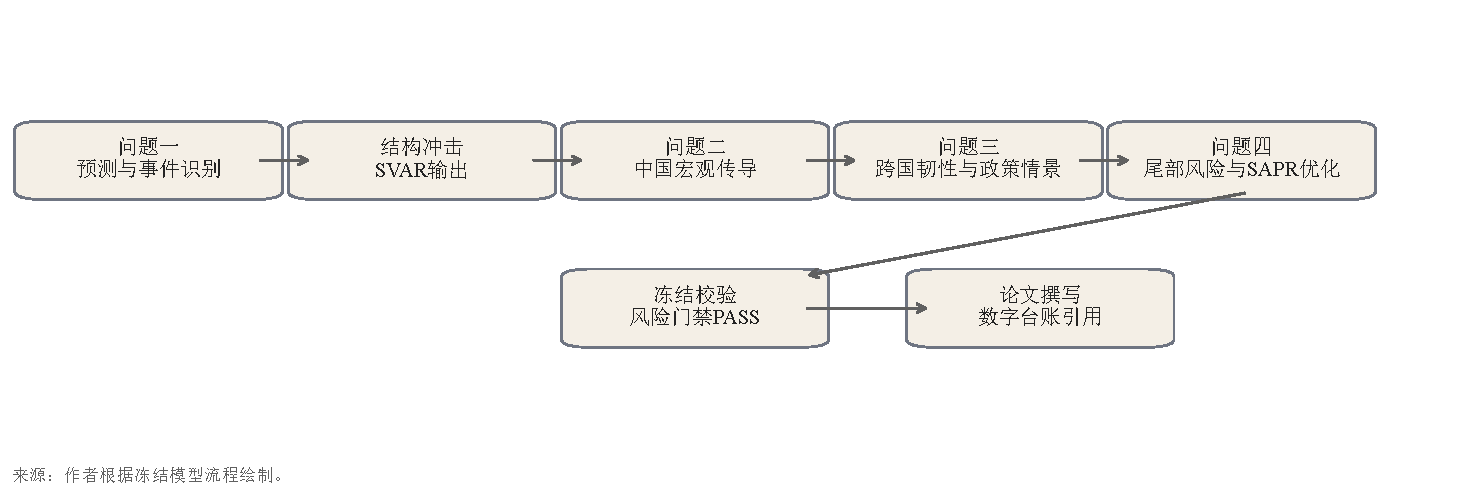
\includegraphics[width=0.92\textwidth]{../figures/paper_route_map.pdf}
  \caption{国际油价冲击研究的总体技术路线}
  \label{fig:route}
\end{figure}

\subsection{数据结构与口径统一}

主样本为2010年1月至2026年6月，共198个月。Brent、WTI、广义美元指数和人民币
汇率由公开日度序列聚合；美国商业原油库存采用月末最后一个已发布周值；GPR使用固定
下载版本的月度指数。中国PPI和规模以上工业增加值来自国家统计局，工业增加值1--2月
合并发布形成的结构性空值原样保留，不作线性插值。人民币原油成本以
``Brent美元价乘人民币兑美元汇率''构造，避免不完整进口单位价值破坏主样本。

跨国部分包含中国、德国、法国、意大利、西班牙、日本和韩国。中国使用受管制汽油标准品
最高零售限价，2013年3月至2026年6月共有160个有效月；欧洲使用含税Euro-super 95，
日本和韩国使用普通汽油全国价格。各币种先与本币Brent配对后取对数变化，从而消除币值
和绝对价格水平差异。整体CPI统一转为同比，工业活动统一使用同比或可比响应。主要公开
数据源与处理见表\ref{tab:data-source}。

\begin{table}[H]
  \centering
  \small
  \caption{核心数据、频率及处理口径}
  \label{tab:data-source}
  \begin{tabularx}{0.98\textwidth}{p{0.19\textwidth}p{0.22\textwidth}p{0.13\textwidth}X}
    \toprule
    数据模块 & 来源 & 原始频率 & 统一处理与用途 \\
    \midrule
    Brent、WTI、汇率 & EIA/FRED\cite{freddata} & 日度 & 交易日事件研究；自然月有效观测均值进入月度模型 \\
    美国商业原油库存 & EIA\cite{eiadata} & 周度 & 月末最后一个已发布周值，防止月内后见信息 \\
    GPR & Caldara--Iacoviello\cite{caldara2022} & 月度 & 使用2026-07-01固定版本，近期值允许后续修订 \\
    中国PPI、IAV、GDP & 国家统计局\cite{nbsdata} & 月/季度 & PPI、IAV进入月度传导；GDP仅作季度验证 \\
    七国CPI、工业活动 & OECD\cite{oecddata} & 月度 & CPI同比与工业活动可比响应；保留方法口径标识 \\
    七国燃油价格 & 各国官方或公开数据中心 & 周/月/事件 & 月均化后与本币Brent对数收益匹配 \\
    中国调价政策 & 国家发展改革委\cite{ndrc2016} & 事件 & 编码机制应调、实际调价及累计未调价差额 \\
    \bottomrule
  \end{tabularx}
\end{table}

所有预测均按时间扩展窗口估计，外生变量至少滞后一期；完整月均值只在月末以后使用。
所有模型共用随机种子20260730。关键结果保存为冻结数值，正文只按预先规定精度展示，
不从图中目测或事后改变口径。

\subsection{四问求解策略}

问题一以no-change为可用基线，将ARIMA、SARIMAX、ETS、Theta和等权组合置于相同
滚动回测中；冲突影响使用交易日累计异常收益、匹配周末安慰剂和GJR--GARCH条件波动率，
历史三类结构冲击则由递归VAR给出。问题二对每个宏观结果变量估计局部投影，并以
ARDL、冲击正负拆分和季度GDP验证稳健性。问题三先做分国分布滞后传导率，再做含国家
与年月固定效应的相对中国面板局部投影，最后关闭临时调控构造价格及宏观反事实。问题四
使用FHS--GJR--GARCH生成条件尾部分布，并在开发样本上枚举三档传导规则，通过四目标
Pareto前沿选择膝点，在隔离检验样本和2026冲击上验证。
